%  LaTeX support: latex@mdpi.com
%  For support, please attach all files needed for compiling as well as the log file, and specify your operating system, LaTeX version, and LaTeX editor.

%=================================================================
% pandoc conditionals added to preserve backwards compatibility with previous versions of rticles

\documentclass[notspecified,article,submit,moreauthors,pdftex]{Definitions/mdpi}


%% Some pieces required from the pandoc template
\setlist[itemize]{leftmargin=*,labelsep=5.8mm}
\setlist[enumerate]{leftmargin=*,labelsep=4.9mm}


%--------------------
% Class Options:
%--------------------

%---------
% article
%---------
% The default type of manuscript is "article", but can be replaced by:
% abstract, addendum, article, book, bookreview, briefreport, casereport, comment, commentary, communication, conferenceproceedings, correction, conferencereport, entry, expressionofconcern, extendedabstract, datadescriptor, editorial, essay, erratum, hypothesis, interestingimage, obituary, opinion, projectreport, reply, retraction, review, perspective, protocol, shortnote, studyprotocol, systematicreview, supfile, technicalnote, viewpoint, guidelines, registeredreport, tutorial
% supfile = supplementary materials

%----------
% submit
%----------
% The class option "submit" will be changed to "accept" by the Editorial Office when the paper is accepted. This will only make changes to the frontpage (e.g., the logo of the journal will get visible), the headings, and the copyright information. Also, line numbering will be removed. Journal info and pagination for accepted papers will also be assigned by the Editorial Office.

%------------------
% moreauthors
%------------------
% If there is only one author the class option oneauthor should be used. Otherwise use the class option moreauthors.

%---------
% pdftex
%---------
% The option pdftex is for use with pdfLaTeX. Remove "pdftex" for (1) compiling with LaTeX & dvi2pdf (if eps figures are used) or for (2) compiling with XeLaTeX.

%=================================================================
% MDPI internal commands - do not modify
\firstpage{1}
\makeatletter
\setcounter{page}{\@firstpage}
\makeatother
\pubvolume{1}
\issuenum{1}
\articlenumber{0}
\pubyear{2023}
\copyrightyear{2023}
%\externaleditor{Academic Editor: Firstname Lastname}
\datereceived{ }
\daterevised{ } % Comment out if no revised date
\dateaccepted{ }
\datepublished{ }
%\datecorrected{} % For corrected papers: "Corrected: XXX" date in the original paper.
%\dateretracted{} % For corrected papers: "Retracted: XXX" date in the original paper.
\hreflink{https://doi.org/} % If needed use \linebreak
%\doinum{}
%\pdfoutput=1 % Uncommented for upload to arXiv.org

%=================================================================
% Add packages and commands here. The following packages are loaded in our class file: fontenc, inputenc, calc, indentfirst, fancyhdr, graphicx, epstopdf, lastpage, ifthen, float, amsmath, amssymb, lineno, setspace, enumitem, mathpazo, booktabs, titlesec, etoolbox, tabto, xcolor, colortbl, soul, multirow, microtype, tikz, totcount, changepage, attrib, upgreek, array, tabularx, pbox, ragged2e, tocloft, marginnote, marginfix, enotez, amsthm, natbib, hyperref, cleveref, scrextend, url, geometry, newfloat, caption, draftwatermark, seqsplit
% cleveref: load \crefname definitions after \begin{document}

%=================================================================
% Please use the following mathematics environments: Theorem, Lemma, Corollary, Proposition, Characterization, Property, Problem, Example, ExamplesandDefinitions, Hypothesis, Remark, Definition, Notation, Assumption
%% For proofs, please use the proof environment (the amsthm package is loaded by the MDPI class).

%=================================================================
% Full title of the paper (Capitalized)
\Title{ProyectoAED2023}

% MDPI internal command: Title for citation in the left column
\TitleCitation{ProyectoAED2023}

% Author Orchid ID: enter ID or remove command
%\newcommand{\orcidauthorA}{0000-0000-0000-000X} % Add \orcidA{} behind the author's name
%\newcommand{\orcidauthorB}{0000-0000-0000-000X} % Add \orcidB{} behind the author's name


% Authors, for the paper (add full first names)
\Author{Carlos$^{}$, Diego$^{}$, Miguel$^{}$}


%\longauthorlist{yes}


% MDPI internal command: Authors, for metadata in PDF
\AuthorNames{Carlos, Diego, Miguel}

% MDPI internal command: Authors, for citation in the left column

% Affiliations / Addresses (Add [1] after \address if there is only one affiliation.)
\address{%
$^{1}$ \quad Universidad de Valencia - ETSE, UV Avinguda de
l'Universitat, 46100 Burjassot,
Valencia; \href{mailto:leutnant@fh-muenster.de}{\nolinkurl{leutnant@fh-muenster.de}}\\
$^{2}$ \quad ; \\
}

% Contact information of the corresponding author
\corres{Correspondence: }

% Current address and/or shared authorship








% The commands \thirdnote{} till \eighthnote{} are available for further notes

% Simple summary
\simplesumm{A Simple summary goes here.}

%\conference{} % An extended version of a conference paper

% Abstract (Do not insert blank lines, i.e. \\)
\abstract{Análisis exploratorio de un conjunto de datos sobre la calidad
del aire de la ciudad de Valencia entre 2004 y 2022}


% Keywords
\keyword{Contaminación, Valencia, datos, Análisis Exploratorio Datos}

% The fields PACS, MSC, and JEL may be left empty or commented out if not applicable
%\PACS{J0101}
%\MSC{}
%\JEL{}

%%%%%%%%%%%%%%%%%%%%%%%%%%%%%%%%%%%%%%%%%%
% Only for the journal Diversity
%\LSID{\url{http://}}

%%%%%%%%%%%%%%%%%%%%%%%%%%%%%%%%%%%%%%%%%%
% Only for the journal Applied Sciences

%%%%%%%%%%%%%%%%%%%%%%%%%%%%%%%%%%%%%%%%%%

%%%%%%%%%%%%%%%%%%%%%%%%%%%%%%%%%%%%%%%%%%
% Only for the journal Data



%%%%%%%%%%%%%%%%%%%%%%%%%%%%%%%%%%%%%%%%%%
% Only for the journal Toxins


%%%%%%%%%%%%%%%%%%%%%%%%%%%%%%%%%%%%%%%%%%
% Only for the journal Encyclopedia


%%%%%%%%%%%%%%%%%%%%%%%%%%%%%%%%%%%%%%%%%%
% Only for the journal Advances in Respiratory Medicine
%\addhighlights{yes}
%\renewcommand{\addhighlights}{%

%\noindent This is an obligatory section in “Advances in Respiratory Medicine”, whose goal is to increase the discoverability and readability of the article via search engines and other scholars. Highlights should not be a copy of the abstract, but a simple text allowing the reader to quickly and simplified find out what the article is about and what can be cited from it. Each of these parts should be devoted up to 2~bullet points.\vspace{3pt}\\
%\textbf{What are the main findings?}
% \begin{itemize}[labelsep=2.5mm,topsep=-3pt]
% \item First bullet.
% \item Second bullet.
% \end{itemize}\vspace{3pt}
%\textbf{What is the implication of the main finding?}
% \begin{itemize}[labelsep=2.5mm,topsep=-3pt]
% \item First bullet.
% \item Second bullet.
% \end{itemize}
%}


%%%%%%%%%%%%%%%%%%%%%%%%%%%%%%%%%%%%%%%%%%


% tightlist command for lists without linebreak
\providecommand{\tightlist}{%
  \setlength{\itemsep}{0pt}\setlength{\parskip}{0pt}}



\usepackage{longtable}
\usepackage{booktabs}
\usepackage{array}
\usepackage{multirow}
\usepackage{wrapfig}
\usepackage{float}
\usepackage{colortbl}
\usepackage{pdflscape}
\usepackage{tabu}
\usepackage{threeparttable}
\usepackage{threeparttablex}
\usepackage[normalem]{ulem}
\usepackage{makecell}
\usepackage{xcolor}

\begin{document}



%%%%%%%%%%%%%%%%%%%%%%%%%%%%%%%%%%%%%%%%%%

\hypertarget{introducciuxf3n}{%
\section{Introducción}\label{introducciuxf3n}}

En el presente informe planteamos el análisis exploratorio de un
conjunto de datos sobre la calidad del aire de la ciudad de Valencia
entre 2004 y 2022. El dataset empleado continene observaciones obtenidas
de distintas estaciones de la red de vigilancia de Valencia. Las
observaciones están compuestas por variables respectivas a diversas
moleculas y elementos presentes en el aire junto a otras de tipo
meteorológico como la velocidad del viento, la temperatura, etc.

El procedimiento a seguir comenzará con la correcta importación del
dataset, a lo que seguirá un previo estudio de los datos con el objetivo
de conocer la estructura del dataset y sus peculiaridades. Continuaremos
con la preparación de los datos para resolver las preguntas planteadas y
escogerán las variables de interés y los periodos temporales sobre los
que se realizará el análisis univariante y bivariante, por otro lado
también se gestionarán los outliers y datos faltantes. ç

Una vez preparado el dataset y estudiadas sus variables, procederemos a
responder a las preguntas planteadas mediante diversas metodologías.
Todo el proceso irá acompañado de las explicaciones pertinentes y
finalizaremos con una conclusión del trabajo realizado.

\hypertarget{objetivos}{%
\section{Objetivos}\label{objetivos}}

El objetivo principal de este trabajo es familizarse con las
herramientas y metodologías aprendidas para la carga, manipulación y
análisis exploratorio de un conjunto de datos. Como objetivos
principales tenemos: analisis univariante y bivariante, detección e
imputación de NA's, detección y gestión de outliers. Por otro lado,
planteamos otros objetivos en forma de preguntas:

\begin{itemize}
\item
  ¿Existe algún tipo de influencia sobre los niveles de gases
  contaminantes debido al cambio en el tráfico hacia el centro (creación
  carriles bici y reducción de carriles) de la ciudad en los últimos
  años?
\item
  ¿Existe alguna correlación entre la calidad del aire y el día de la
  semana/año?
\item
  ¿Existe cierta evolución de la contaminación sonora (años/zonas)?
\item
  ¿Existe cierta evolución de la temperatura? (A medias, se puede hacer
  algo más o incluso relacionarlo con las precipitaciones. No se me
  ocurre cómo pero se le podría dar una vuelta)
\item
  ¿Existe cierta evolución de la contaminación. Como medir la
  contaminación?
\end{itemize}

\hypertarget{anuxe1lisis-exploratorio-de-los-datos}{%
\section{Análisis exploratorio de los
datos}\label{anuxe1lisis-exploratorio-de-los-datos}}

\hypertarget{importaciuxf3n-de-los-datos}{%
\subsection{Importación de los
datos}\label{importaciuxf3n-de-los-datos}}

Para la importación de nuestro dataset fue necesario establecer ``;''
como el separador de las variables. Por otro lado, definimos el formato
de las variables de forma previa ya que tras una exploración visual
percibimos variables de tipo \emph{factor} y \emph{fecha}. Con el
objetivo de estudiar las características generales de nuestro dataset
realizamos un sumario con el tipo de cada variable \emph{type}, cuantos
valores distintos tiene \emph{levels}, su valor más frecuente
\emph{topLevel}, cuántas veces aparece \emph{topCount}, y en qué
proporción \emph{topFreq} y por último la proporción de datos faltantes
de cada variable \emph{missFreq}. En el Anexo 1, en la Tabla
\ref{tabla:anexo1}, encontramos las características generales obtenidas.
A contrinuación explicamos cada variable:

\begin{itemize}
\item
  \emph{Id} es un identificador para cada una de las filas y no aporta
  ninguna información concreta.
\item
  \emph{Fecha} es una variable tipo \emph{Date} que nos proporciona la
  fecha en la que se tomaron los datos que componen la observación.
  Tomaremos esta variable para la ordenación ascendente de los datos.
\item
  \emph{Dia\_de\_la\_semana} y \emph{Dia\_del\_mes} son variables de
  tipo factor que indican en que día de la semana y en qué día del mes
  se realiza la medida. Puede ser extraído a partir de \emph{Fecha}
  usando las funciones \emph{wday()} y \emph{day()}, de la librería
  \emph{lubridate}.
\item
  \emph{Estacion} es una variable de tipo factor cuyos niveles son las
  distintas estaciones meteorológicas donde se tomaron las mediciones de
  las variables numéricas, haciendo un total de 13 estaciones.
\item
  \emph{PM1, PM2.5, PM10} son variables de tipo numérico con datos sobre
  la concentración de materiales particuldos (PM) de menos de 1, 2.5 y
  10 micrómetros de diámetro respectivamente.
\item
  \emph{NO, NO2, NOx, O2, SO2, CO, NH3} son variables con datos sobre la
  concentración de estas moléculas inorgánicas consideradas
  contaminantes en el aire. Respecto a los óxidos de nitrógeno (NOx),
  estos son un grupo de gases compuestos por oxígeno y nitrógeno, es
  decir, NO y NO2 forman parte de este grupo y por lo tanto los valores
  de las variables estarán altamente correlacionados.
\item
  \emph{C7H8, C6H6, C8H10} son variables con datos sobre la
  concentración de estas moléculas orgánicas también consideradas
  contaminantes en el aire.
\item
  \emph{Vel\_viento, Dir\_viento, Temperatura, Humidad\_rel, Presion,
  Radiacion\_solar, Precipitacion, Max\_vel\_viento} son variables
  numéricas con mediciones de estas distintas condiciones ambientales al
  momento de medir las concentraciones de moléculas contaminantes en el
  aire.
\item
  \emph{As, Ni, Cd, Pb} son variables numéricas con datos de otras
  concentraciones de gases y metales contaminantes en el aire.
\item
  \emph{B(a)p} es una variable booleana que sólo presenta una
  observación. Elresto de datos son faltants y no podemos saber lo que
  representa esta variable.
\item
  \emph{Fecha\_creación} y \emph{Fecha\_baja} son variables de tipo
  \emph{Date} que parecen estar relacionadas con la creacion del dataset
  y que no parecen aportar información sobre nuestros datos.
  \emph{Fecha\_creación} solo presenta dos entradas distintas y
  \emph{Fecha\_baja} sólo presenta NA's por lo que estas variables
  parecen prescindibles.
\end{itemize}

En el sumario mencionado anteriormente se pueden observar grandes
porcentajes de NA's en todas las variables. Esto junto al conocimiento
de que los datos provienen de distintas estaciones, nos hace pensar que
el dataset está compuesto por la unión de diversos datasets de los que
provienen las mismas o distintas variables. En la siguiente sección
vamos a analizar más profundamente los datos faltantes.

\hypertarget{anuxe1lisis-de-datos-faltantes-y-especiales}{%
\subsection{Análisis de datos faltantes y
especiales}\label{anuxe1lisis-de-datos-faltantes-y-especiales}}

En esta sección, previamente al análisis univariante y bivariante de las
variables, vamos a realizar un análisis más profundo de la estructura
del dataset. El dataset parece estar compuesto por la unión de un
conjunto datasets, posiblemente por las distintas estaciones de las que
provienen los datos. Con el objetivo de obtener un conjunto de datos
consistente, analizaremos el porcentaje de NA's que hay por cada
variable, luego veremos que datos proporcionan las estaciones y con que
frecuencia, también comprobaremos cuando comenzaron a generar datos las
estaciones y durante que periodos de tiempo se han obtenido las
variables.

En el Anexo 1, en la Tabla \ref{tabla:anexo1} podemos confirmar los
elevados porcentajes NA's. Para comprobar el origen de los NA's en el
mapa de calor de la Figura \ref{fig:mapa_calor}, podemos ver qué
variables mide cada estación meteorológica, además de la cantidad de
datos que aporta cada una de ellas sobre cada varaible numérica. Con
este gráfico verificamos cada estación obtiene conjuntos distintos de
variables y con frecuencias distintas, lo que hace pensar que las
variables se toman en distintos periodos de tiempo.

Como podemos ver en la Figura \ref{fig:estaciones_activas}, las
estaciones se van incorporando al estudio con el paso del tiempo, esto
explica la diferencia de observaciones obtenida por cada una de ellas.
Por otro lado, nos interesa saber durante que periodos de tiempo se
obtienen las variables. A partir del gráfico de la Figura
\ref{fig:periodos_variables} podemos ver el periodo de tiempo en el que
las variables comienzan a ser medidas. Tras esta primera visualización
de nuestros datos, podemos concluir que la gran cantidad de datos
faltantes se debe a una combinación del hecho de que no todas las
estaciones miden todas las variables, sumado a que los datos de ciertas
variables se empiezan a medir posteriormente que el resto.

En nuestro caso vamos a escoger un período de 10 años, desde 2012 a
2022, ya que en este período de tiempo hay un número significativo de
estaciones recogiendo datos y la mayoría de las variables son medidas en
este intervalo de tiempo de forma consistente. No obstante, decidimos
descartar las variables \emph{Pb}, \emph{Cd}, \emph{Ni}, \emph{As},
\emph{B(a)p} y \emph{NH3} debido a que se comienzan a medir después del
2012 y resultaría poco razonable imputar los datos de estas variables en
esos años. De la misma forma, también descartamos las variables
\emph{C7H8}, \emph{C6H6}, y \emph{C8H10} debido a que presentan grandes
períodos de tiempo con ausencia de datos intercalados entre 2012 y 2022,
por lo que también sería poco razonable imputar estos datos.

\begin{figure}

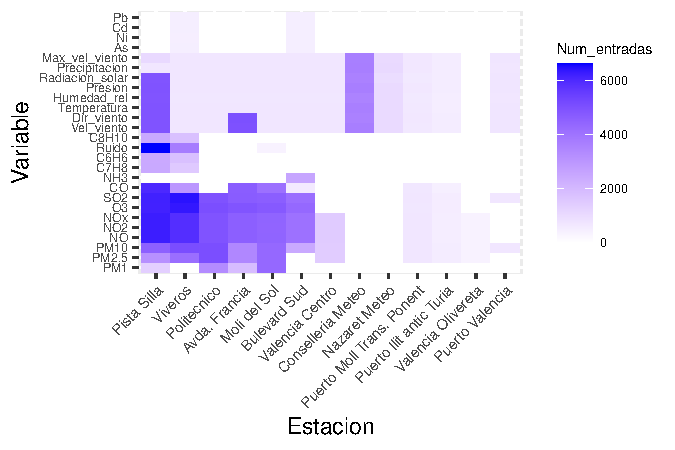
\includegraphics[width=0.7\linewidth]{ProyectoAED2023_files/figure-latex/mapa_calor-1} \hfill{}

\caption{\label{fig:mapa_calor}}\label{fig:mapa_calor}
\end{figure}

\begin{figure}

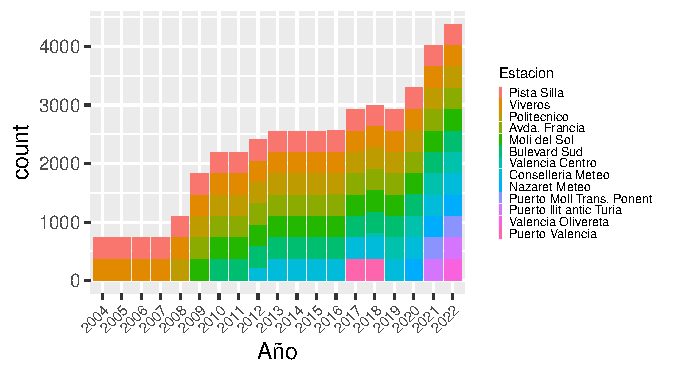
\includegraphics[width=0.7\linewidth]{ProyectoAED2023_files/figure-latex/estaciones_activas-1} \hfill{}

\caption{\label{fig:estaciones_activas}}\label{fig:estaciones_activas}
\end{figure}

\begin{figure}

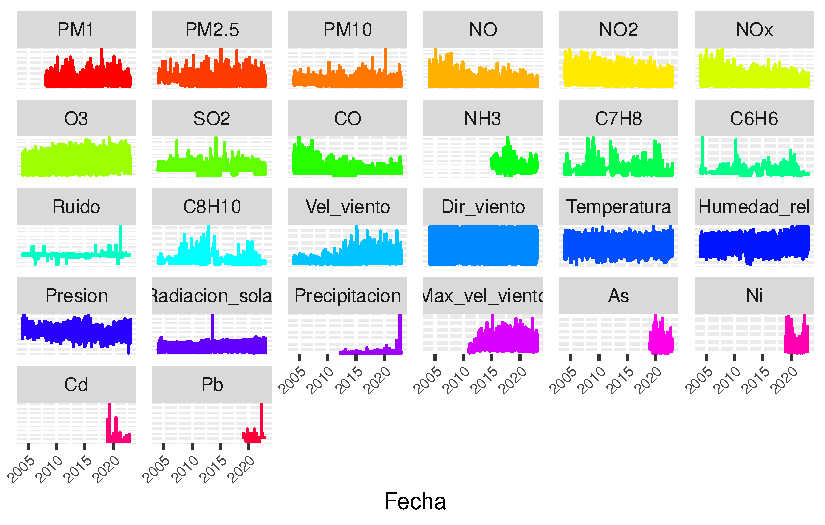
\includegraphics[width=0.7\linewidth]{ProyectoAED2023_files/figure-latex/periodos_variables-1} \hfill{}

\caption{\label{fig:periodos_variables}}\label{fig:periodos_variables}
\end{figure}

\hypertarget{anuxe1lisis-univariante}{%
\subsection{Análisis univariante}\label{anuxe1lisis-univariante}}

\hypertarget{caracteruxedsticas-univariantes}{%
\subsubsection{Características
univariantes}\label{caracteruxedsticas-univariantes}}

En esta sección analizaremos las variables de interés de forma
individual con el objetivo de conocer sus magnitudes, es decir, las
unidades de medida que representan, y como se distribuyen. Comenzamos
con un summary de las variables numéricas para analizar sus magnitudes y
como se distribuyen los datos. El resultado de este sumario lo podemos
ver en el Anexo 1 Tabla \ref{tabla:anexo3}. Mediante el sumario anterior
podemos averiguar cuales son las unidades de medida empleadas
contrastando con información externa, ya que en la fuente de los datos
no se proporcionan.

\begin{itemize}
\tightlist
\item
  Gases (NO, NO2, NOx, SO2, CO, O3): microgramos por metro cubico
  (\(\mu\)g/m3)
\item
  Temperatura: grados centígrados (Cº)
\item
  Humedad: porcentaje (\%)
\item
  Presión: hectopascales (hPa)
\item
  Velocidad del viento: kilometros/hora (m/s)
\item
  Dirección del viento: ángulo de 0 a 360 (º)
\item
  Precipitación: litros de agua por metro cuadrado (mm)
\item
  Radiación solar: Vatios por metro cuadrado (W/m2)
\item
  Ruido: decibelios (dB)
\end{itemize}

También es interesante observar las distribuciones de estas variables.
Esto podemos observarlo en las figuras \ref{fig:densidades1} y
\ref{fig:densidades2}.

\begin{figure}

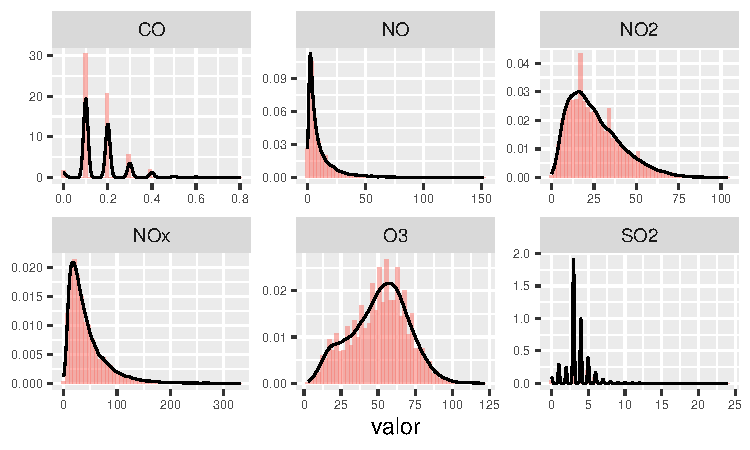
\includegraphics[width=0.7\linewidth]{ProyectoAED2023_files/figure-latex/densidades1-1} \hfill{}

\caption{\label{fig:densidades1}}\label{fig:densidades1}
\end{figure}

\begin{figure}

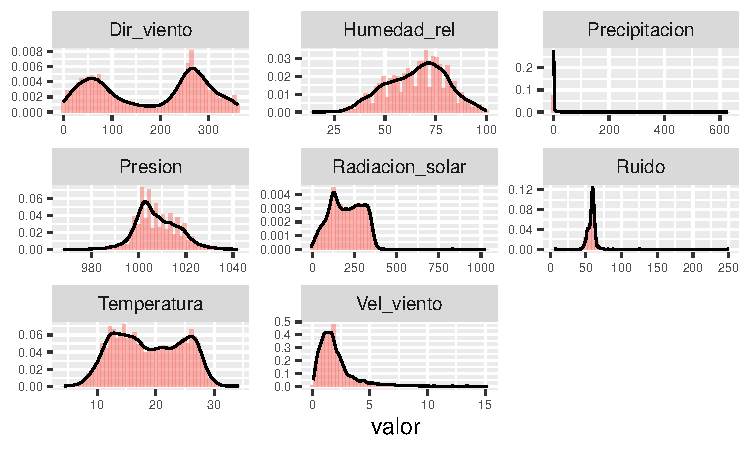
\includegraphics[width=0.7\linewidth]{ProyectoAED2023_files/figure-latex/densidades2-1} \hfill{}

\caption{\label{fig:densidades2}}\label{fig:densidades2}
\end{figure}

\hypertarget{detecciuxf3n-y-eliminaciuxf3n-de-outliers-con-muxe9todos-univariantes}{%
\subsubsection{Detección y eliminación de outliers con métodos
univariantes}\label{detecciuxf3n-y-eliminaciuxf3n-de-outliers-con-muxe9todos-univariantes}}

Compararemos el funcionamiento de lass reglas tresSigma, hampel, boxplot
y percentiles. En la Figura \ref{fig:outliers_univ} podemos observar
cómo la regla del percentil siempre elimina datos (el 2.5\% superior e
inferior). Podemos usar esto como comparador de el resto de métodos. Es
visible el agresivo comportamiento de la regla boxplot y el
excesivamente poco agresivo método de la regla 3-sigma. Hemos decidido
utilizar la regla de Hampel para la detección de los outliers, ya que
esta es una regla robusta a distribuciones que no sean Gaussianas. En
cuanto a qué hacer con estos outliers, hemos decidido sustituirlos por
NA para su posterior inputación.

\begin{figure}

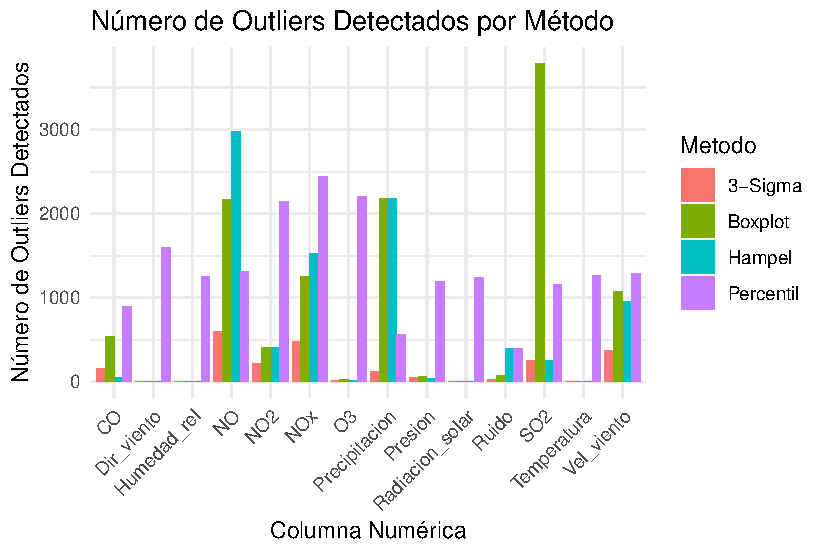
\includegraphics[width=0.7\linewidth]{ProyectoAED2023_files/figure-latex/ourliers_univ-1} \hfill{}

\caption{\label{fig:outliers_univ}}\label{fig:ourliers_univ}
\end{figure}

\hypertarget{analisis-bivariante}{%
\subsection{Analisis bivariante}\label{analisis-bivariante}}

\hypertarget{caracteruxedsticas-bivariantes}{%
\subsubsection{Características
bivariantes}\label{caracteruxedsticas-bivariantes}}

Mediante boxplots vamos a analizar como se distribuyen los datos
respecto a las estaciones. En la figura \ref{fig:boxplot_est1} se
observan las referentes a gases y en la figura \ref{fig:boxplot_est2} el
resto. A partir de ambas figuras podemos concluir con que generalmente
la estación no influye en los valores de las variables. Esta información
nos es útil para la imputación de NA's, ya que podemos emplear datos de
otras estaciones.

\begin{figure}

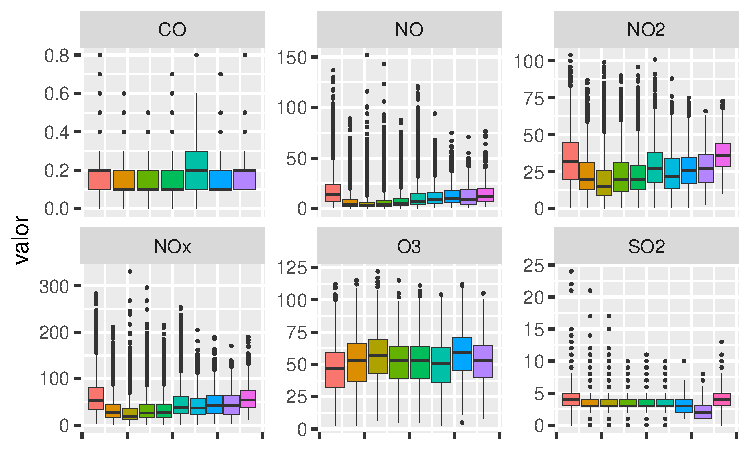
\includegraphics[width=0.7\linewidth]{ProyectoAED2023_files/figure-latex/boxplot_est1-1} \hfill{}

\caption{\label{fig:boxplot_est1}}\label{fig:boxplot_est1}
\end{figure}

\begin{figure}

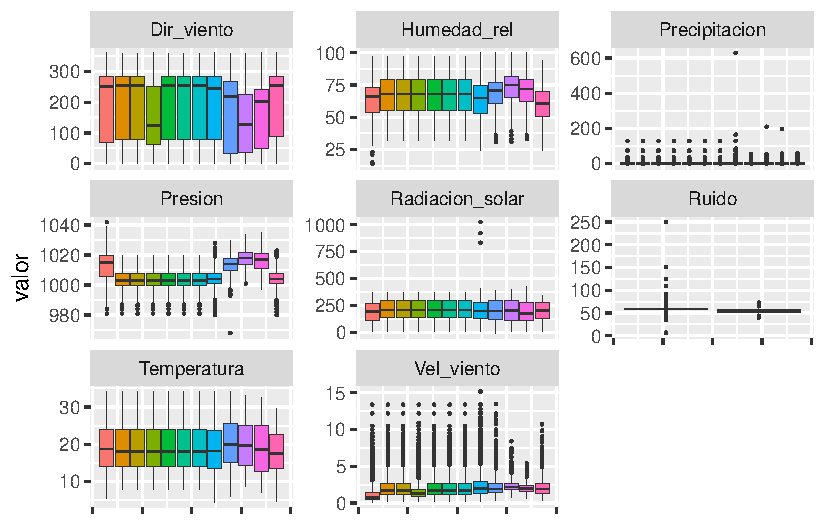
\includegraphics[width=0.7\linewidth]{ProyectoAED2023_files/figure-latex/boxplot_est2-1} \hfill{}

\caption{\label{fig:boxplot_est2}}\label{fig:boxplot_est2}
\end{figure}

También visualizaremos la evolución mediante boxplots de el valor de las
variables a lo largo de los años. En la Figura \ref{fig:boxplot_anos1}
se puede apreciar una leve reducción a lo largo de los años de los gases
considerados como contaminantes a excepción del SO2 que parece
mantenerse constante. Por otro lado vemos un leve aumento del ozono
(O3), por lo que podría existir una relación con la disminución de gases
contaminantes. Continuamos con las variables meteorológicas. Como era de
esperar, en la Figura \ref{fig:boxplot_anos2} vemos como las variables
meteorológicas no han sufrido variaciones a lo largo de los años. Por
otro lado si que se aprecia un leve aumento en el ruido.

\begin{figure}

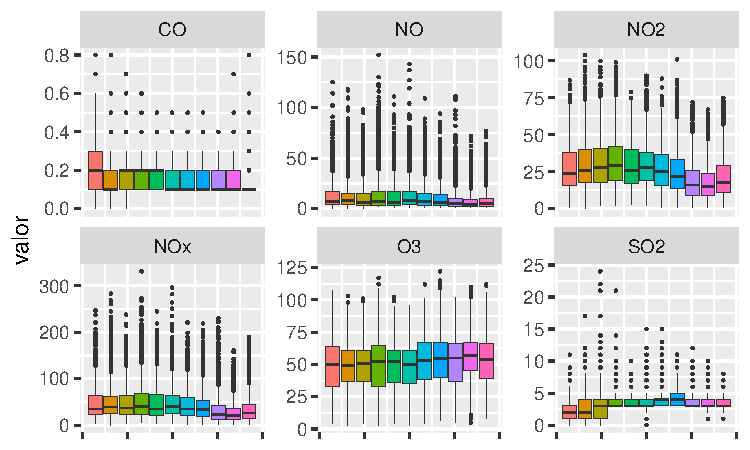
\includegraphics[width=0.7\linewidth]{ProyectoAED2023_files/figure-latex/boxplot_anos1-1} \hfill{}

\caption{\label{fig:boxplot_anos1}}\label{fig:boxplot_anos1}
\end{figure}

\begin{figure}

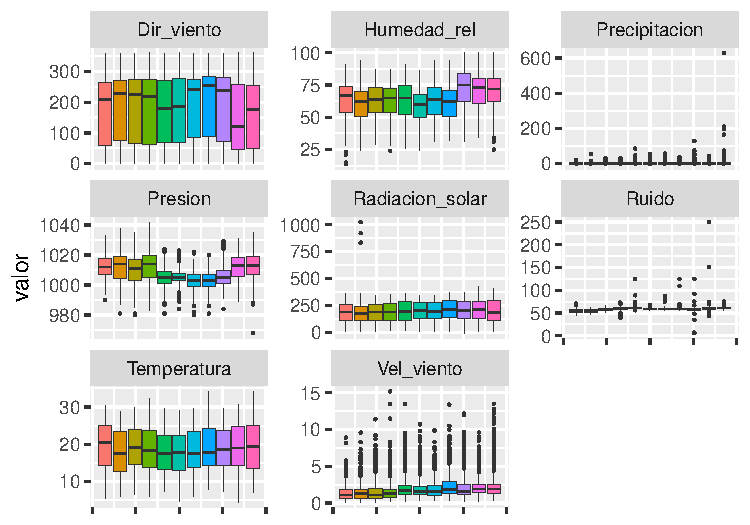
\includegraphics[width=0.7\linewidth]{ProyectoAED2023_files/figure-latex/boxplot_anos2-1} \hfill{}

\caption{\label{fig:boxplot_anos2}}\label{fig:boxplot_anos2}
\end{figure}

\hypertarget{imputaciuxf3n-de-datos-anuxf3malos}{%
\subsubsection{Imputación de datos
anómalos}\label{imputaciuxf3n-de-datos-anuxf3malos}}

Ahora que conocemos las unidades de nuestras variables tras haberlas
analizado, sabemos cuál es el rango de valores puede tomar cada una.
Para tratar estos datos anómalos, en primer lugar se convertirán en NA's
y a continuación se les imputará un valor igual que el resto de datos
faltantes. En el anáslisis univariante vimos que los datos diarios de
las variables en todas las estaciones de Valencia suelen ser parecido.
Decidimos usar este hecho para imputar los datos faltantes en cada día
con la media de esta variable sobre todas las estaciones.

\hypertarget{correlaciones}{%
\subsubsection{Correlaciones}\label{correlaciones}}

Basándonos en la Figura \ref{fig:correlaciones1}, podemos extraer las
siguientes conclusiones:

\begin{itemize}
\item
  Existe una correlación negativa importante entre NOs y Ozono. Esto
  podría deberse a que la presencia de óxidos de nitrógeno puede
  contribuir a la degradación del ozono en la atmósfera, lo que tiene
  implicaciones para la calidad del aire, la contaminación y el efecto
  hivernadero.
\item
  Correlación positiva de NOx con el resto de NO (NO, NO2\ldots). Como
  era de esperar y como se ha mencionado en la definición de las
  variables, NOx representa el conjunto de oxidos de nitrogeno, entre
  ellos el NO y el NO2.
\item
  Correlación positiva entre Temperatura y Radiación Solar. Esto es
  coherente con las estaciones más cálidas que a menudo experimentan más
  horas de sol y mayor radiación solar.
\item
  Correlación entre Radiación Solar y Ozono. Esto tiene sentido ya que
  la capa de ozono filtra la mayor parte de la radiación ultravioleta
  proveniente del sol, por lo tanto están muy relacionados entre ellos.
\end{itemize}

\begin{figure}

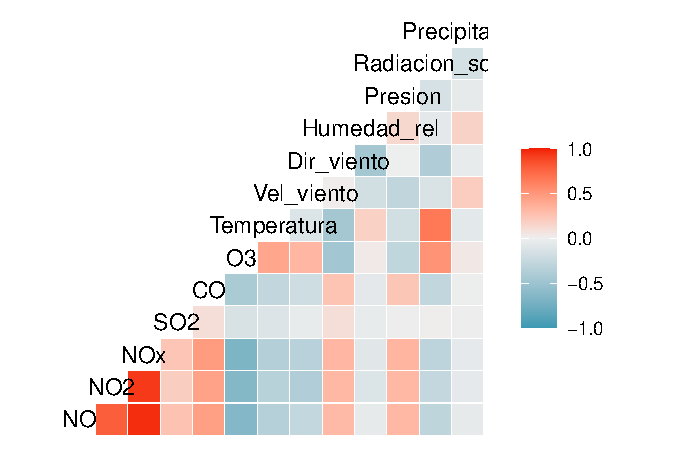
\includegraphics[width=0.7\linewidth]{ProyectoAED2023_files/figure-latex/correlaciones1-1} \hfill{}

\caption{\label{fig:correlaciones1}}\label{fig:correlaciones1}
\end{figure}

\hypertarget{detecciuxf3n-y-eliminaciuxf3n-de-outliers-con-muxe9todos-multivariable}{%
\subsubsection{Detección y eliminación de outliers con métodos
multivariable}\label{detecciuxf3n-y-eliminaciuxf3n-de-outliers-con-muxe9todos-multivariable}}

La distancia de Mahalanobis mide la distancia de un punto de datos a un
conjunto de datos multivariado centrado y escalado según la matriz de
covarianza. Los puntos que tienen distancias de Mahalanobis más grandes
son considerados como outliers, ya que están más lejos de la
distribución típica de los datos. En otras palabras: con estos métodos
multivariable no nos fijamos en que un valor sea anómalo, sino una
combinación de estos, siendo representados en un espacio vectorial y
midiendo la distancia de cada punto (muestra) con el resto. Lo que
haremos al encontrar un outlier será eliminarlo directamente, pues toda
la muestra será anómala.

\hypertarget{resoluciuxf3n-de-preguntas-planteadas-sobre-los-datos}{%
\section{Resolución de preguntas planteadas sobre los
datos}\label{resoluciuxf3n-de-preguntas-planteadas-sobre-los-datos}}

\hypertarget{influencia-de-carril-bici}{%
\subsection{Influencia de carril bici}\label{influencia-de-carril-bici}}

Para estudiar la influencia de un carril bici por el centro de Valencia,
estudiaremos la evolución de gases contaminantes en diversas estaciones
de la ciudad. Mediremos la evolución de los gases SO2 y NO2,
relacionados con la combustión de carburantes fósiles, el tráfico rodado
y las emisiones de determinadas industrias y grandes instalaciones de
combustión. Además, las estaciones deberían ser las más céntricas, ya
que ahí el efecto del carril bici y las restricciones de acceso deberían
hacerse más notables. Observaremos las siguientes estaciones: Avda.
Francia, Bulevard Sud, Valencia Centro y Olivereta

Si bien, en la Figura \ref{fig:pregunta1_1} no se observan cambios
significativos en los niveles de SO2, en la Figura \ref{fig:pregunta1_2}
sí que podemos observar una evolución en los niveles de NO2 a lo largo
de los años. Los niveles más bajos se dan en los últimos 3 años. Además,
se puede apreciar una reducción periódica de los niveles de NO2 en los
meses de verano, que coincide con el momento del año donde menos gente
vive en la ciudad y menos tráfico hay. En conclusión parece que las
medidas de transporte que se han tomado en la ciudad han influenciado en
la reducción de gases contaminantes.

\begin{figure}

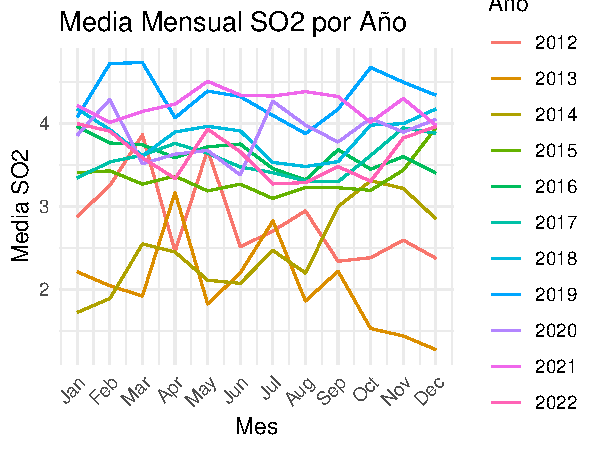
\includegraphics[width=0.7\linewidth]{ProyectoAED2023_files/figure-latex/pregunta1_1-1} \hfill{}

\caption{\label{fig:pregunta1_1}}\label{fig:pregunta1_1}
\end{figure}

\begin{figure}

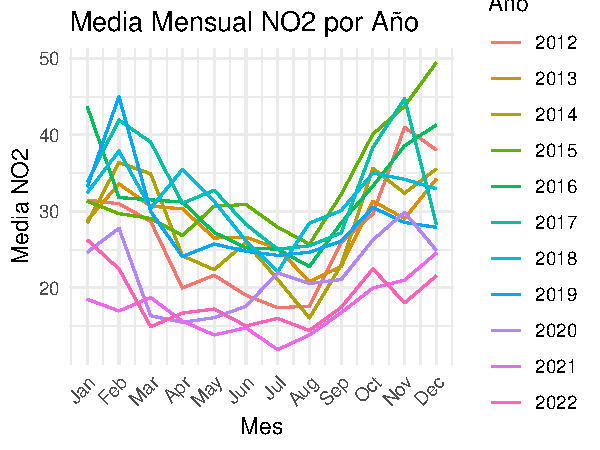
\includegraphics[width=0.7\linewidth]{ProyectoAED2023_files/figure-latex/pregunta1_2-1} \hfill{}

\caption{\label{fig:pregunta1_2}}\label{fig:pregunta1_2}
\end{figure}

\hypertarget{relaciuxf3n-entre-la-calidad-del-aire-y-el-dia-de-la-semana}{%
\subsection{Relación entre la calidad del aire y el dia de la
semana}\label{relaciuxf3n-entre-la-calidad-del-aire-y-el-dia-de-la-semana}}

En esta pregunta observamos si, en general la calidad del aire se ve
influenciada por el día de la semana. Queremos sobre todo fijarnos en la
distinción entre días laborables y de descanso. Podemos comprobar cómo,
efectivamente, existe una disminución en los gases contaminantes los
días festivos con respecto a los días laborables.

\begin{figure}

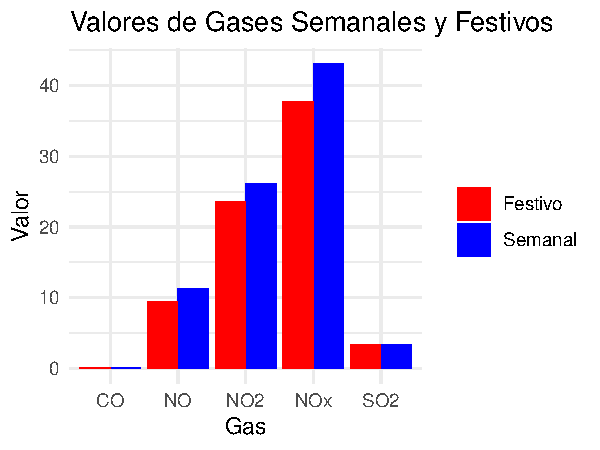
\includegraphics[width=0.7\linewidth]{ProyectoAED2023_files/figure-latex/pregunta2-1} \hfill{}

\caption{\label{fig:pregunta2}}\label{fig:pregunta2}
\end{figure}

\hypertarget{evoluciuxf3n-de-la-contaminaciuxf3n-sonora-a-lo-largo-de-los-auxf1os}{%
\subsection{Evolución de la contaminación sonora a lo largo de los
años}\label{evoluciuxf3n-de-la-contaminaciuxf3n-sonora-a-lo-largo-de-los-auxf1os}}

En la Figura \ref{fig:pregunta3_1} podemos observar un incremento en el
ruido medio a lo largo de los años. En los datos del 2020 podemos
observar un decrecimiento de los mismos. Podría estudiarse si este
efecto es debido al Covid-19.

Con la figura \ref{fig:pregunta3_2} comprobaremos si este ruido medido
depende de la zona dónde la midamos. Podemos observar que la desviación
es despreciaable. Sí que podemos determinar, gracias a contrastar estos
datos con los de la gráfica boxplot \ref{boxplot_anos2}, es que la
evolución en el ruido no viene dada por una tendencia natural. Más bien,
el gráfico nos indica que existe un aumento significativo de ruido en
días concretos.

\begin{figure}

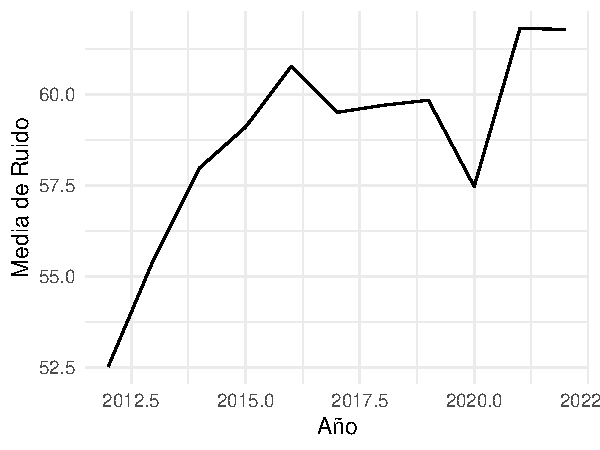
\includegraphics[width=0.7\linewidth]{ProyectoAED2023_files/figure-latex/pregunta3_1-1} \hfill{}

\caption{\label{fig:pregunta3_1}}\label{fig:pregunta3_1}
\end{figure}

\begin{figure}

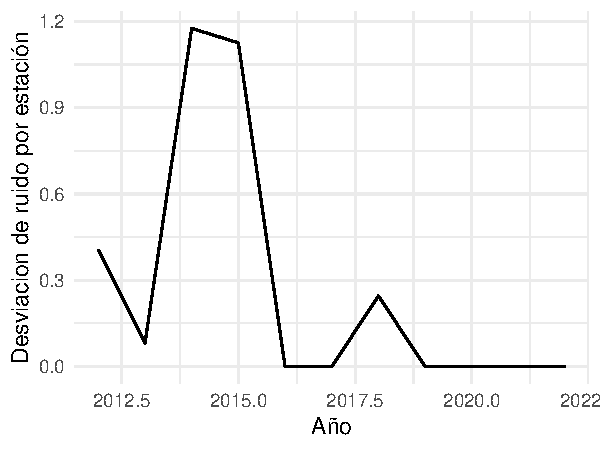
\includegraphics[width=0.7\linewidth]{ProyectoAED2023_files/figure-latex/pregunta3_2-1} \hfill{}

\caption{\label{fig:pregunta3_2}}\label{fig:pregunta3_2}
\end{figure}

\hypertarget{evoluciuxf3n-de-la-temperatura-a-lo-largo-de-los-auxf1os}{%
\subsection{Evolución de la temperatura a lo largo de los
años}\label{evoluciuxf3n-de-la-temperatura-a-lo-largo-de-los-auxf1os}}

En la Figura \ref{fig:pregunta4} se puede observar el aumento
generalizado de la temperatura a lo largo de los años. Es curioso que,
pese a que en el mundo existe un aumento generalizado de la temperatura,
en Valencia estuvo bajando esta tendencia y no es hasta el año 2017 que
comenzaron a subir de nuevo. Pese a lo mencionado, bastante visible el
hecho de que nos encontramos en una tendencia creciente.

\begin{figure}

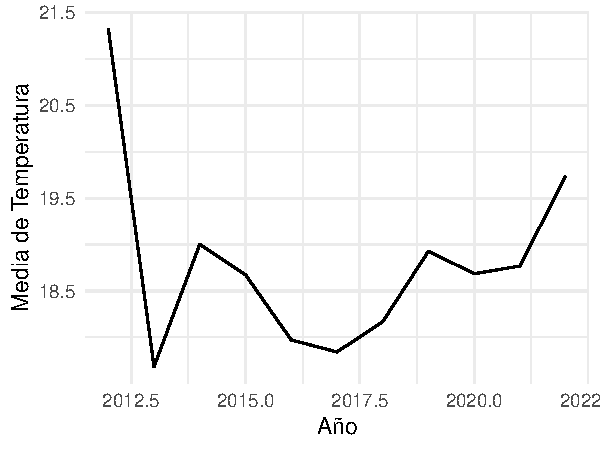
\includegraphics[width=0.7\linewidth]{ProyectoAED2023_files/figure-latex/pregunta4-1} \hfill{}

\caption{\label{fig:pregunta4}}\label{fig:pregunta4}
\end{figure}

\hypertarget{cuxf3mo-se-ha-comportado-la-contaminaciuxf3n-a-lo-largo-de-los-auxf1os}{%
\subsection{Cómo se ha comportado la contaminación a lo largo de los
años}\label{cuxf3mo-se-ha-comportado-la-contaminaciuxf3n-a-lo-largo-de-los-auxf1os}}

Estudiaremos el comportamiento de todos los gases contaminantes en todas
las estaciones. Gracias a superponer todas estas evoluciones en un mismo
gráfico, podemos tomar perspectiva y comparar el comportamiento entre
los diferentes gases.

Esta vez, en la Figrua \ref{fig:pregunta5} podemos que en general las
medidas de estos se han mantenido bastante estables o decrecientes en el
tiempo. Con las gráficas de la figura \ref{boxplot_anos1} podemos
contrastar la información que nos otorga esta gráfica. Por ejemplo:

\begin{itemize}
\tightlist
\item
  El CO sí parece decrecer en el último año. Sin embargo, por los
  outliers y el rango de valores que se maneja, en el gráfico presente
  puede no apreciarse esta evolución.
\item
  Por ejemplo, en evoluciones como la del NO2 podemos reforzar la
  fiabilidad observando cómo la tendencia en su representación de
  boxplot es similar. Incluso parece haber consistencia en los datos que
  la regla boxplot marca como outliers.
\item
  En el gas SO2, observamos una tendencia estable a lo largo de los
  años. No obstante, comparando con su contraparte representada en
  boxplot ganamos la información de que el gas ha ido ganando
  estabilidad, habiendo cada vez menos outliers con el paso del tiempo.
\end{itemize}

\begin{figure}[H]

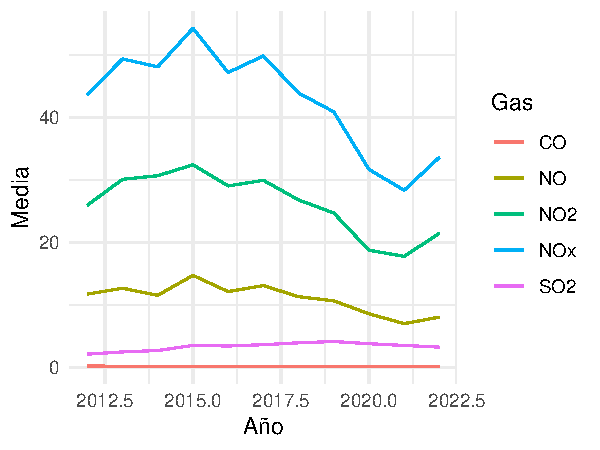
\includegraphics[width=0.7\linewidth]{ProyectoAED2023_files/figure-latex/pregunta5-1} \hfill{}

\caption{\label{fig:pregunta5}}\label{fig:pregunta5}
\end{figure}

\hypertarget{conclusion}{%
\section{Conclusion}\label{conclusion}}

En definitiva, a lo largo de este análisis hemos utilizado métodos de
exploración visual para ayudarnos a comprender la estructura interna de
nuestros datos. También se ha realizado un análisis univariante de las
variables obteniendo estadísticos que nos ayudaron averiguar sus
unidades de medida, las cuales eran previamente desconocidas. También se
han determinado relaciones entre nuestras variables en el análisis
bivariante, que pueden servir para plantear estudios futuros. Además,
utilizando la información obtenida durante el análisis se han descartado
algunas variables y se han imputado los valores anómalos del resto.
Finalmente, se han respondido algunas preguntas que surgieron durante el
proceso de análisis utilizando un dataset sin valores anómalos.

\hypertarget{Anexo}{%
\section{Anexo 1}\label{Anexo}}

\begin{table}[H]

\caption{\label{tab:unnamed-chunk-4}Sumario variables\label{tabla:anexo1}}
\fontsize{7}{9}\selectfont
\begin{tabular}[t]{ccccccc}
\toprule
variable & type & levels & topLevel & topCount & topFrec & missFrec\\
\midrule
Id & numeric & 43388 & 1 & 1 & 0 & 0\\
Fecha & Date & 6940 & 2022-01-01 & 12 & 0 & 0\\
Dia\_de\_la\_semana & factor & 7 & Sabado & 6205 & 0.143 & 0\\
Dia\_del\_mes & factor & 31 & 16 & 1426 & 0.033 & 0\\
Estacion & factor & 13 & Pista Silla & 6940 & 0.16 & 0\\
\addlinespace
PM1 & numeric & 179 & 4 & 978 & 0.023 & 0.748\\
PM2.5 & numeric & 221 & 9 & 1567 & 0.036 & 0.463\\
PM10 & numeric & 479 & 13 & 1104 & 0.025 & 0.336\\
NO & numeric & 178 & 2 & 3890 & 0.09 & 0.23\\
NO2 & numeric & 120 & 16 & 961 & 0.022 & 0.23\\
\addlinespace
NOx & numeric & 338 & 21 & 647 & 0.015 & 0.23\\
O3 & numeric & 116 & 56 & 688 & 0.016 & 0.241\\
SO2 & numeric & 22 & 3 & 15273 & 0.352 & 0.237\\
CO & numeric & 18 & 0.1 & 7358 & 0.17 & 0.548\\
NH3 & numeric & 21 & 5 & 469 & 0.011 & 0.941\\
\addlinespace
C7H8 & numeric & 235 & 1 & 163 & 0.004 & 0.908\\
C6H6 & numeric & 76 & 1 & 370 & 0.009 & 0.902\\
Ruido & numeric & 67 & 62 & 1135 & 0.026 & 0.751\\
C8H10 & numeric & 182 & 1 & 240 & 0.006 & 0.901\\
Vel\_viento & numeric & 117 & 0.9 & 972 & 0.022 & 0.535\\
\addlinespace
Dir\_viento & numeric & 362 & 264 & 177 & 0.004 & 0.536\\
Temperatura & numeric & 282 & 16.5 & 146 & 0.003 & 0.637\\
Humedad\_rel & numeric & 82 & 71 & 521 & 0.012 & 0.644\\
Presion & numeric & 64 & 1002 & 850 & 0.02 & 0.634\\
Radiacion\_solar & numeric & 401 & 139 & 104 & 0.002 & 0.639\\
\addlinespace
Precipitacion & numeric & 209 & 0 & 9545 & 0.22 & 0.73\\
Max\_vel\_viento & numeric & 397 & 3.5 & 335 & 0.008 & 0.724\\
As & numeric & 50 & 0.28 & 288 & 0.007 & 0.978\\
Ni & numeric & 405 & 0.75 & 11 & 0 & 0.978\\
Cd & numeric & 64 & 0.03 & 124 & 0.003 & 0.978\\
\addlinespace
Pb & numeric & 6 & 0.01 & 929 & 0.021 & 0.978\\
B(a)p & logical & 2 & FALSE & 1 & 0 & 1\\
Fecha\_creacion & Date & 2 & 2022-12-04 & 39008 & 0.899 & 0\\
Fecha\_baja & Date & 1 & NA & 0 & 0 & 1\\
\bottomrule
\end{tabular}
\end{table}

\begin{table}[H]

\caption{\label{tab:unnamed-chunk-10}Sumario de variables numericas\label{tabla:anexo3}}
\fontsize{7}{9}\selectfont
\begin{tabular}[t]{lccccccccc}
\toprule
  & min & Q1.25\% & median & mean & dt & Q3.75\% & max & n & IQR\\
\midrule
NO & 0.0 & 3.0 & 6.0 & 10.83 & 13.36 & 13.0 & 152.0 & 25107 & 10.0\\
NO2 & 0.0 & 14.0 & 22.0 & 25.58 & 15.42 & 35.0 & 104.0 & 25105 & 21.0\\
NOx & 0.0 & 18.0 & 32.0 & 41.93 & 33.85 & 55.0 & 331.0 & 25107 & 37.0\\
SO2 & 0.0 & 3.0 & 3.0 & 3.40 & 1.43 & 4.0 & 24.0 & 24064 & 1.0\\
CO & 0.0 & 0.1 & 0.1 & 0.16 & 0.09 & 0.2 & 0.8 & 12261 & 0.1\\
\addlinespace
O3 & 3.0 & 38.0 & 53.0 & 50.83 & 19.15 & 64.0 & 122.0 & 23958 & 26.0\\
Temperatura & 4.4 & 13.9 & 18.5 & 18.86 & 5.75 & 24.1 & 34.2 & 12950 & 10.2\\
Vel\_viento & 0.1 & 1.0 & 1.6 & 2.01 & 1.56 & 2.4 & 15.2 & 16261 & 1.4\\
Dir\_viento & 0.0 & 67.0 & 220.0 & 179.31 & 110.28 & 274.0 & 360.0 & 16226 & 207.0\\
Humedad\_rel & 14.0 & 55.0 & 67.0 & 65.81 & 14.51 & 76.0 & 100.0 & 12652 & 21.0\\
\addlinespace
Presion & 968.0 & 1002.0 & 1007.0 & 1007.73 & 8.56 & 1014.0 & 1042.0 & 13037 & 12.0\\
Radiacion\_solar & -7.0 & 126.0 & 200.0 & 200.75 & 94.03 & 281.0 & 1025.0 & 12841 & 155.0\\
Precipitacion & 0.0 & 0.0 & 0.0 & 1.26 & 8.93 & 0.0 & 629.0 & 11725 & 0.0\\
Ruido & 6.0 & 55.0 & 59.0 & 58.08 & 6.77 & 61.0 & 250.0 & 5157 & 6.0\\
\bottomrule
\end{tabular}
\end{table}

%%%%%%%%%%%%%%%%%%%%%%%%%%%%%%%%%%%%%%%%%%

\vspace{6pt}

%%%%%%%%%%%%%%%%%%%%%%%%%%%%%%%%%%%%%%%%%%
%% optional

% Only for the journal Methods and Protocols:
% If you wish to submit a video article, please do so with any other supplementary material.
% \supplementary{The following supporting information can be downloaded at: \linksupplementary{s1}, Figure S1: title; Table S1: title; Video S1: title. A supporting video article is available at doi: link.}

%%%%%%%%%%%%%%%%%%%%%%%%%%%%%%%%%%%%%%%%%%







%%%%%%%%%%%%%%%%%%%%%%%%%%%%%%%%%%%%%%%%%%
%% Optional

%% Only for journal Encyclopedia


%%%%%%%%%%%%%%%%%%%%%%%%%%%%%%%%%%%%%%%%%%
%% Optional
%%%%%%%%%%%%%%%%%%%%%%%%%%%%%%%%%%%%%%%%%%
\begin{adjustwidth}{-\extralength}{0cm}

%\printendnotes[custom] % Un-comment to print a list of endnotes



% If authors have biography, please use the format below
%\section*{Short Biography of Authors}
%\bio
%{\raisebox{-0.35cm}{\includegraphics[width=3.5cm,height=5.3cm,clip,keepaspectratio]{Definitions/author1.pdf}}}
%{\textbf{Firstname Lastname} Biography of first author}
%
%\bio
%{\raisebox{-0.35cm}{\includegraphics[width=3.5cm,height=5.3cm,clip,keepaspectratio]{Definitions/author2.jpg}}}
%{\textbf{Firstname Lastname} Biography of second author}

%%%%%%%%%%%%%%%%%%%%%%%%%%%%%%%%%%%%%%%%%%
%% for journal Sci
%\reviewreports{\\
%Reviewer 1 comments and authors’ response\\
%Reviewer 2 comments and authors’ response\\
%Reviewer 3 comments and authors’ response
%}
%%%%%%%%%%%%%%%%%%%%%%%%%%%%%%%%%%%%%%%%%%
\PublishersNote{}
\end{adjustwidth}


\end{document}
